% Preliminary Requirements for openETCS --- WP2
% Author: Sylvain Baro (SNCF)
% Version 1.0.0


\documentclass{template/openetcs_article}
% Use the option "nocc" if the document is not licensed under Creative Commons
%\documentclass[nocc]{template/openetcs_article} 
\usepackage{rotating,url,color}
\graphicspath{{./template/}{.}{./images/}}
\begin{document}
\frontmatter
\project{openETCS}

%Please do not change anything above this line
%============================
% The document metadata is defined below

%assign a report number here
\reportnum{OETCS/WP2/D2.6~--~01.00.00}

%define your workpackage here
\wp{Work-Package 2: ``Requirements''}

%set a title here
\title{Preliminary Requirements for openETCS}

%set a subtitle here
%\subtitle{A template for short document. Adapted from report template.}

%set the date of the report here
\date{March 2013}

%define a list of authors and their affiliation here

\author{Sylvain Baro}
\affiliation{SNCF}
  
  
% define the coverart
\coverart[width=350pt]{chart}

%define the type of report
\reporttype{Requirements}




%
% End of QA Zone
\begin{abstract}
This document provides a preliminary view of the requirements for the openETCS project. 
It is meant to evolve after the initial release in order to provide the full requirement lists.
\end{abstract}

%=============================
%Do not change the next three lines
\maketitle

% 
% QA zone

\begin{tabular}{|p{4.4cm}|p{8.7cm}|}
\hline
\multicolumn{2}{|c|}{Document information} \\
\hline
Work Package &  WP2  \\
Deliverable ID or doc. ref. & D2.6\\
\hline
Document title & Preliminary Requirements for openETCS \\
Document version & 01.00.00 \\
Document authors (org.)  & Sylvain Baro (SNCF) \\
\hline
\end{tabular}

\begin{tabular}{|p{4.4cm}|p{8.7cm}|}
\hline
\multicolumn{2}{|c|}{Review information} \\
\hline
Last version reviewed & 00.01.00 \\
\hline
Main reviewers & St\'ephane Callet, Cyril Cornu, David Mentre, Marielle Petit-Doche, Stanislas Pinte, Merlin Pokam, Guillaume Pottier, Uwe Steinke\\
\hline
\end{tabular}

\begin{tabular}{|p{2.2cm}|p{4cm}|p{4cm}|p{2cm}|}
\hline
\multicolumn{4}{|c|}{Approbation} \\
\hline
  &  Name & Role & Date   \\
\hline  
Written by    &  Sylvain Baro &   & \\
\hline
Approved by & Gilles Dalmas & WP2 leader & \\
\hline
\end{tabular}

\begin{tabular}{|p{2.2cm}|p{2cm}|p{3cm}|p{5cm}|}
\hline
\multicolumn{4}{|c|}{Document evolution} \\
\hline
Version &  Date & Author(s) & Justification  \\
\hline  
00.00.00 & 01/01/13 & S. Baro &  Document creation  \\
\hline  
00.01.00 & 15/01/13 & S. Baro &  Request for comment to some partners, version for review  \\
\hline  
01.00.00 & 05/03/13 & S. Baro &  Version after first review. Req. version is 1. \\
\hline
\end{tabular}

\newpage

\tableofcontents
%\listoffiguresandtables
\newpage





%=============================
% The actual document starts below this line
%=============================


%%%%%%%%%%%%%%%%%%%%%%%%%%%%%%%%%%%%%%%%%%%%%%%%%%%%%%%%%%%%%%
%%%              My macros (=> Sylvain Baro)               %%%
%%%%%%%%%%%%%%%%%%%%%%%%%%%%%%%%%%%%%%%%%%%%%%%%%%%%%%%%%%%%%%
\newcommand{\tbd}{\colorbox{cyan}{\%\%To Be Defined\%\%}}
\newcommand{\tbc}{\colorbox{cyan}{\%\%To Be Confirmed\%\%}}
\newcommand{\todo}[1]{\colorbox{cyan}{\%\%{#1}\%\%}}
\newlength{\origindent}

\newenvironment{issue}{
	\begin{quote}
	\begin{itshape}Open Issue. 
}{
	\end{itshape}
	\end{quote}
}

\newenvironment{comment}{
	\begin{quote}
	\begin{itshape}Comment. 
}{
	\end{itshape}
	\end{quote}
}

\newenvironment{justif}{
	\begin{quote}
	\begin{itshape}Justification. 
}{
	\end{itshape}
	\end{quote}
}
%% Requirements.


\newcounter{reqnum}
\setcounter{reqnum}{0}
\newcounter{subreqnum}
\newcounter{subsubreqnum}
\newlength{\partopbuf}
\newlength{\topbuf}

% Automated numbering versions of the macros
\newcommand{\req}[1]{\addtocounter{reqnum}{1} \setcounter{subreqnum}{0}
	\begin{description}\item[{\small\reqt-X-\thereqnum}] #1\end{description}
}

\newcommand{\subreq}[1]{
	\addtocounter{subreqnum}{1} \setcounter{subsubreqnum}{0}
	\addtolength{\leftmargini}{1cm}
	\begin{description}
	\item[\hspace{0.5cm}{\small\reqt-X-\thereqnum.\thesubreqnum}] #1
	\end{description}
	\addtolength{\leftmargini}{-1cm}
}

\newcommand{\subsubreq}[1]{
	\addtocounter{subsubreqnum}{1}
	\addtolength{\leftmargini}{2cm}
	\begin{description}
	\item[\hspace{1cm}{\small\reqt-X-\thereqnum.\thesubreqnum.\thesubsubreqnum}] #1
	\end{description}
	\addtolength{\leftmargini}{-2cm}
}

% Fixed version of the commands
\newcommand{\reqfixed}[3]{\addtocounter{reqnum}{1} \setcounter{subreqnum}{0}
	\begin{description}\item[{\small\reqt-#1-#2}] #3\end{description}
}

\newcommand{\subreqfixed}[4]{
	\addtocounter{subreqnum}{1} \setcounter{subsubreqnum}{0}
	\addtolength{\leftmargini}{1cm}
	\begin{description}
	\item[\hspace{0.5cm}{\small\reqt-#1-#2.#3}] #4
	\end{description}
	\addtolength{\leftmargini}{-1cm}	
}

\newcommand{\subsubreqfixed}[5]{
	\addtocounter{subsubreqnum}{1}
	\addtolength{\leftmargini}{2cm}
	\begin{description}
	\item[\hspace{1cm}{\small\reqt-#1-#2.#3.#4}] #5
	\end{description}
	\addtolength{\leftmargini}{-2cm}	
}

% Citation of the requirement

% Citation of the reference (for markup purpose)
%\newcommand{\refreq}[1]{\textbf{#1}}

% Citation of the reference and text (for markup purpose)
% The purpose of this is to automatically replace the placeholder by the 
% full text. \fullrefreq{R-xxx}{} or \fullrefreq{R-xxx}{blabla} 
% will be replaced by \fullrefreq{R-xxx}{text of the R-xxx requirement} 
%\newcommand{\fullrefreq}[2]{\textbf{#1}: \textrm{#2}}


\def\reqt{R-WP2/D2.6}
% Start here


\section{Introduction}
The purpose of this document is to enumerate the meta-requirements of the projects: \emph{i.e.} 
the requirements on the modeling, processes, toolchain, validation and verification. The purpose of this document is 
not to provide the system and safety requirements that will specify the model/software 
developed in the OpenETCS project.

The requirements found in the 50126 and 50128 are not rewritten here. The required plans for the 
project (see Sect. \ref{standards}) shall be written according to what is required in the standards,
then reviewed. Once this task is done, the plans will be the reference for the project.
In the meantime, one can refer to the standards, or to the D2.2 document.

This document is initiated as a preliminary requirement list, and will evolve during the project 
to be completed with all the requirements on the methodology
modelling, process, tool chain, and safety proof. The table herebelow sums up the area of responsibility
of the contributors of WP2 on these requirements.


\begin{tabular}{|l|l|l|}
\hline
Subtask ID & Requirements & Subtask leader \\
\hline
D2.6 & Set of requirements on modeling & TUBS  \\
\hline
D2.7 & Set of requirements on API & ALSTOM  \\
\hline
D2.8 &  Set of requirements on tools & ERTMS Solutions  \\
\hline
D2.9 & Set of requirements on V\&V & SNCF \\ 
\hline
\end{tabular}

\section{Reference documents}
\subsection{Standards \& ERA documents}
\begin{itemize}
\item CENELEC EN 50126-1 --- 01/2000 --- \emph{Railways applications –- The specification and 
demonstration of Reliability, Availability, Maintenability and Safety (RAMS) –- Part 1: 
Basic requirements and generic process}
\item CENELEC EN 50128 --- 10/2011 --- \emph{Railway applications -- Communication, signalling and 
processing systems -- Software for railway control and protection systems}
\item CENELEC EN 50129 --- 05/2003 --- \emph{Railway applications –- Communication, signalling and 
processing systems –- Safety related electronic systems for signalling}
\item CCS TSI --- \emph{ CCS TSI for HS and CR transeuropean rail has been adopted by a Commission Decision 2012/88/EU on the 25th January 2012}
\item SUBSET-026 3.3.0 --- \emph{System Requirement Specification}
\item SUBSET-076-x 2.3.y --- Test related ERTMS documentation
\item SUBSET-088 2.3.0 --- \emph{ETCS Application Levels 1 \& 2 - Safety Analysis}
\item SUBSET-091 3.2.0 --- \emph{Safety Requirements for the Technical Interoperability
of ETCS in Levels 1 \& 2}
\end{itemize}
\subsection{Project documents}
\begin{itemize}
\item FPP --- \emph{Project Outline Full Project Proposal Annex OpenETCS} -- v2.2
\item D2.1 --- \emph{Report on existing methodologies} --- Jan Welte and Hansj\"org Manz
\item D2.2 --- \emph{Report on CENELEC standards} --- Merlin Pokam and Norbert Sch\"afer
\end{itemize}

\section{Conventions}
The requirements are prefixed by “R-zz-x-y”, and are written in a roman typeface, where ``R'' 
stands for ``Requirement'', ``zz'' identifies the source document,``x'' 
is the version number and``y'' is the identifier of the requirement. All the text 
written in italics is not a requirement: it may be a note, an open issue, an 
explanation of the requirements, or an example.

The placeholder “\todo{xxx}” is used to indicates that a paragraph or section is not finished, 
to be defined or to be confirmed.

\section{Glossary}
\begin{description}
\item[API] Application Programming Interface
\item[FME(C)A] Failure Mode Effect (and Criticity) Analysis
\item[I/O] Input/Output
\item[OBU] OnBoard Unit
\item[QA] Quality Assurance
\item[RBC] Radio Block Center
\item[RTM] RunTime Model
\item[SIL] Safety Integrity Level
\item[SRS] System Requirement Specification
\item[SSRS] SubSystem Requirement Specification
\item[THR] Tolerable Hazard Rate
\item[V\&V] Verification \& Validation
\end{description}

\section{Goals}
\subsection{Goal 1: Formalization of the SRS in an executable formal and high level model}
The first goal of the project is to propose a formalization of a subset of the on-board subsystem,
as defined in the SUBSET-026, for the chosen reference baseline. 

The purpose of the formalization is:
\begin{itemize}
\item to enhance the understanding of modelled subset;
\item to allow formal analysis of the modelled subset;
\item to be able to animate the model for testing and analyzing purpose;
\item to provide information on the completeness and soundness of the SUBSET-026;
\item to be used as a reference formal specification for the implementation of an OBU 
(by the OpenETCS project team and by industrial actors);
\item \dots
\end{itemize}

In order to conduct this formalization, a part of the tool chain and methodology defined (see Goal 2) 
will be used.

The output of this goal is a formal specification, translatable to other tools (SCADE, 
Simulink, B tools, OpenETCS tool chain\dots) that can be given to all railway actors, and 
if possible associated to SRS documents in the ERA database.

The final goal is that industrial actors work with this formal specification instead of 
natural language specification.

\subsection{Goal 2: Definition of a process/methodologies for developing 
on onboard software that can fulfill the EN 50128 requirements}

This process/methodology must allow to produce SIL4 software.
The full safety process needed for the OpenETCS to be \emph{certifiable} according to CENELEC 50126
and 50128 shall be described in details. This safety plan will detail precisely which activities 
are required or not, why, and the choices that are made that allows to claim that safety is guaranteed.

Because the full design, development, validation and safety analysis process for a SIL4 OBU
is a huge task far beyond the project possibilities, the full safety activities will not be conducted
on the whole subsystem (see below). Nevertheless the safety process description shall be complete 
according to CENELEC requirements.

The process has to ensure that toolchain, formalized SUBSET-026 specification and models are certifiable 
according to these standards while emerging from an open source environment. 

\subsection{Goal 3: Definition of a tool chain for developing 
on onboard software that can fulfill the EN 50128 requirements}

These tools must be ``certifiable'' according to the corresponding tool level of EN 50128 (considering the 
process for which they are used), but will not be certified as part of the project.

By the combination of Goal 1, 2 and 3, it should be possible for the industry to build an ETCS 
onboard software:
\begin{itemize}
\item By using OpenETCS model and proving the implementation satisfies the model;
\item By using the OpenETCS toolchain with their own model;
\item By using the OpenETCS model and toolchain.
\end{itemize}

\subsection{Goal 4: Building an implementation of the subset of an onboard ETCS using the model and the 
tool chain defined in Goal 1 \& 2}

It is the demonstration that all the work done in the OpenETCS project is coherent, and that
the tool chain is operational.

\subsection{Goal 5: Define the safety properties at the model level}
In order to comply the CENELEC standards, it is necessary to conduct safety activities 
to identify errors and anomalies in the process. One important step for this is to define safety 
properties which are on the same level than the formal model.

These safety properties:
\begin{itemize}
\item will be used for the validation of the model itself;
\item will be used as reference proof obligations for the subsequent activies.
\end{itemize}

However the full safety analysis is out of the scope of the OpenETCS project. 
We will consider that SUBSET-088 and SUBSET-091 will provide the roots 
elements for safety analysis, and this elements will be refined and allocated into the modelled 
subsystem. 

Please note that this is unsufficient in order to guarantee the safety of a system that would embed an OpenETCS 
OBU. The complete assertion of safety is not in the scope of the project.

\subsection{Goal 6: Provide a subset of the safety case}
Selected part of the safety process shall be applied (either by applying the full process on a small
subset of the development, or by applying a part of the activities on the whole project development).

\subsection{Goal 7: Promote OpenETCS}
Promote this work to push it to become a \emph{de facto} standard for the industrial actors, 
(like \emph{e.g.} the AUTOSAR standard in the automotive world).

\section{Project outline}
In order to pursue these goals, the development cycle for the project may be presented as follow. 

\textbf{Please note that this is just an outline of the activities, not the project plan, nor the 
Q\&A, nor the Validation plan. The verification arrows where not represented on this outline in order 
not to clutter the drawing. Also note that the activities needed for the toolchain are not
covered here.}

Fig. \ref{fig:main_process} shows the main part of the development process. This process may be seen
as a ``triple-V''. The smaller V corresponds to the development of the formal model. 

It starts by the SRS which is not part of the project (SUBSET-026), then outlines the boundaries and 
the applicable requirements from the SUBSET-026 that will be used in the formal model. This outline 
is provided in the Subsystem Requirement Specification. This document describe the subsystem that 
will be modelled. It describes the architecture of the subsystem (functions and their I/O) and the 
requirements allocated to these functions. If necessary, the requirements are rewritten in order to 
address the I/O and to correspond to the allocation. This document also provide the Safety/Non Safety 
classification of the requirements. The architecture part is described in a formal or semi-formal 
language, and the requirements are described in natural language.

The next step is the creation of the formal model itself, from the SSRS. Because this model is executable, 
it can be validated as itself, thus the first ``closing branch'' of the V.

From the model can be derived some ``abstract'' code. The word ``abstract'' is used to emphasize that 
this code is not necessarily capable of running on a full SIL4 platform. This code can be validated 
in the second ``closing branch'', possibly using some of the work done in the first branch. 

A project demonstrator may be derived from this code (or may be the ``abstract'' code itself).

The third ``closing branch'' corresponds to the production of code capable of running on a 
given SIL4 platform, and the associated validation activities. This is not part of the project.

The yellow boxes correspond to activities that should be covered completely in order to produce 
a certifiable product, but of which only a subset will be conducted in order to demonstrate the 
capabilities of the product. We consider that doing the full set of activities for the project to 
be fully compliant to CENELEC standards (\emph{i.e.} to be certifiable) is a huge task. Hence we 
should isolate a subset of this tasks, as complete in terms of tasks as possible in order to be 
convinced of the feasibility of the whole activities. 

Therefore we have to discriminate three kinds of tasks:
\begin{description}
\item[blue:] the tasks that will be completely achieved in the scope of the OpenETCS project;
\item[red:] the tasks that will be not be achieved, because they are out of the scope of the OpenETCS project;
\item[yellow:] the tasks for which a sample will be achieved, because they are in the scope of the 
OpenETCS but doing them completely is unrealistic considering the resources of the project.
\end{description}

\begin{figure}
  \centering
  \fbox{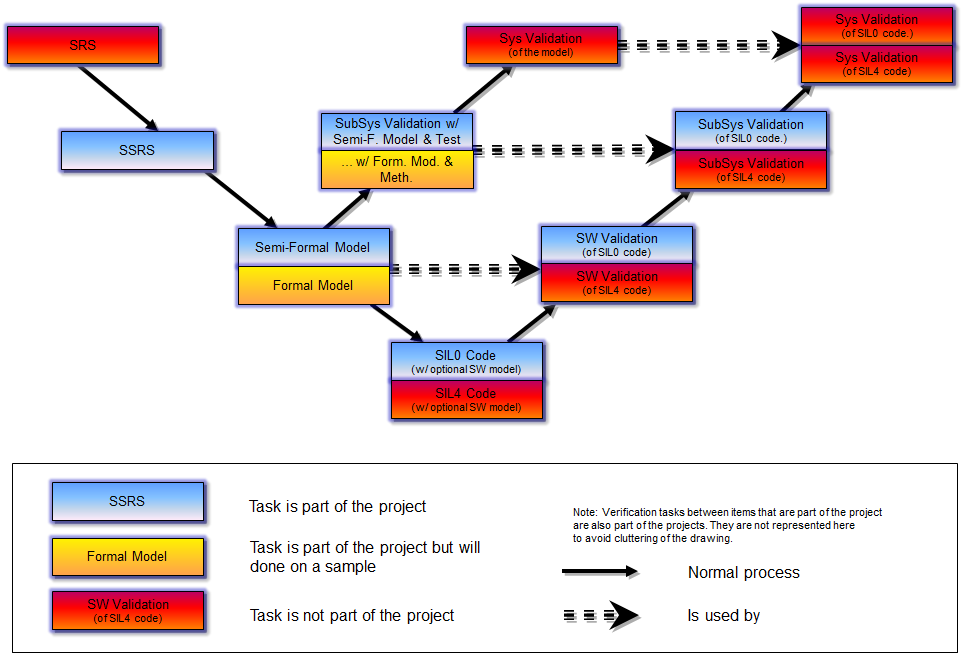
\includegraphics[scale=0.65]{Process1.png}}
  \caption{Main process}
  \label{fig:main_process}
\end{figure}

Fig. \ref{fig:safety_process} shows activities that are needed for the safety analyses. It should 
be considered in parallel of the descending branch of the V, but has been put on a separate diagram for
the sake of clarity. The validation tasks corresponds to the safety validation of the model w.r.t. 
the safety properties. Verification tasks corresponds to the verification that the properties are each
step are correct and complete w.r.t. the higher level properties. Indeed for both these tasks, arrows should 
really be bidirectional.

High level safety properties are provided, which must be refined side-to-side with each step on the 
descending branch of the V. These properties are then used for the safety analysis of the model. The 
validation (safety analyses) boxes are yellow because the full activity will not be conducted. Only 
a subset of the safety properties will be proved.

\begin{figure}
  \centering
  \fbox{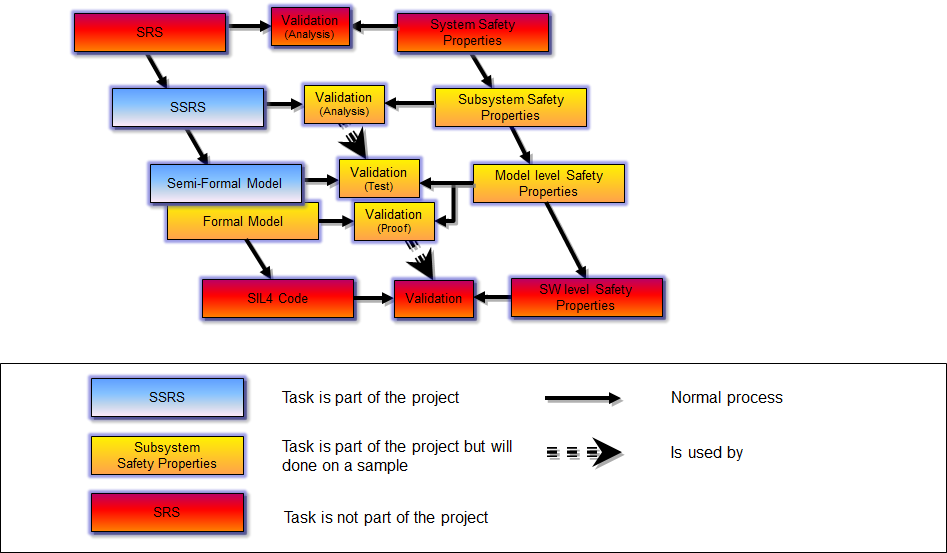
\includegraphics[scale=0.80]{Process2.png}}
  \caption{Safety analyses}
  \label{fig:safety_process}
\end{figure}

Regarding the process, WP2 shall issue (through this document) the requirements on V\&V, including
safety activities. From these requirements, WP4 shall propose the corresponding plans (Safety,
Verification and Validation). This plans will then be reviewed by WP2 to check conformance to the 
requirements. The reviewed plans will then be used as reference for the activities of the WPs.


\section{Requirements}
\subsection{Standards}
\label{standards}

\reqfixed{01}{001}{The project shall comply the CENELEC EN 50126, 50128 and 50129 standards.}
\begin{comment}
This requirements pull some documentation issue (for example a project plan 
and a safety plan\,\footnote{Each plan is in the scope of the Work Package responsible for the 
corresponding tasks. \emph{I.e.} V\&V plan shall be issued by WP4.} which describe what to do in the 
context of an Open Source critical software), but it also pull other requirements (compliance to 
ISO~9001, skill of the people in contact with critical items). These points must be 
considered\,\footnote{The plan has to describe either how the requirement is applied in the context
of OpenETCS project, or why it is not needed.} in the QA Plan.

EN~50129 goes down to the hardware, but it also provides information on the system safety activities. 
In the scope of the project (which does not include the hardware), we will follow the EN~50129 for the components 
which are within the scope, and justify that some activities are not conducted because they corresponds
to items outside this scope. 
\emph{E.g.} we do not have an implementation on a real hardware, therefore we will not require to go as down as safety 
analysis of the hardware itself. Hence the scope of the safety activities must be provided clearly in the safety plan, 
and will exclude some activities as ``out of scope''. Nevertheless this is not equivalent to only applying EN~50128.
\end{comment}


\subreqfixed{01}{001}{01}{A QA Plan shall be issued and complied with.}
\subreqfixed{01}{001}{02}{The QA Plan shall describe the management of versions, OpenETCS baselines, 
connexion with ERTMS baselines, project life cycle, maintenance and evolution plan, organisation and roles.}
\subreqfixed{01}{001}{03}{A Verification plan shall be issued and complied with.}
\subreqfixed{01}{001}{04}{A Validation Plan shall be issued and complied with.}
\subreqfixed{01}{001}{05}{The techniques applied to the software will be compliant regarding the SIL.}
\subreqfixed{01}{001}{06}{All the output documents required by the EN~50126, EN~50128 and EN~50129 for 
each step of the lifecycle shall be issued, or their lack of shall be justified.}
\subreqfixed{01}{001}{07}{The tools used shall be developed in order to be certifiable according to EN 50128.}

\begin{comment}
No requirement on the way of doing this. \emph{E.g.} to have a certified 
(certifiable?) code generator, two generators and comparison of the result, one
 generation and one verification chain\dots
 \end{comment}



\reqfixed{01}{002}{All Roles, responsabilities and more generally participators to any task (development, documentation, 
validation\dots) on any step of the project development shall be tracked, in particular
to show independence of the development and testing teams. The way of tracking shall be explained in
the QA Plan.}

\subsection{Runtime Model \& API}
The framework needs to provide a list of properties and functions. If we take the parallel of the Java environment, some of these properties/functions will be 
provided by the \emph{abstract machine} properties, and some of them will be provided by the API.

If we consider for example ``allocation of memory'', in Java usually it is just provided by the creation of an object (thus in the ``Runtime model''). In C it is given by the 
\emph{malloc} function, which is part of the API (of course, we will find eventually that it leads to the runtime model too, but in the user point of view, it is
definitely part of the API).

What I consider is that at requirement level, we do not want to know which property will come from API and whichm will come from the runtime model. We are only
interested in the properties themselves.

In order to avoid ambiguities, we will define the following.
\begin{description}
\item[Runtime model.] This is the abstract layer required to ``run'' the formal model. It shall provide
in the formalism part or all of the following (but not restricted to):
\begin{itemize}
\item memory management,
\item execution of state machines (or of the chosen formal objects), 
\item failures, 
\item communication between processes and concurrence. 
\end{itemize}
All these can be provided with or without safety properties. This corresponds in fact to the services 
provided by the ``abstract machine(s)'' which runs the models.
\item[API.]
 This is the functions/primitives required to complete the \emph{Runtime model}. It shall provide
the remaining of the features listed hereabove which are not provided by the Runtime model.

All these can be provided with or without safety properties.
\item[RTM/API.]
This corresponds to the Runtime Model \emph{plus} API. Therefore it should provide all the services
needed to emulate at abstract level the hardware platform that could run the software.
\item[Functional Architecture.] This corresponds to the functional boundaries between the ETCS KERNEL 
and the other functional components (JRU, DMI, Odometry, Eurobalise, Euroradio\dots). These boundaries
are described in the FIS or FFFIS. It also includes the parting of the KERNEL into different 
functions.
\end{description}

In the following requirements, we will not discriminate what is required from the API and from the 
RTM. This is the definition of these components that will allocate the requirements to the different 
parts. Hence we will only state requirements on the RTM/API.

\subsubsection{RTM/API}
\textbf{This chapter has to be completed by the leader of D2.7}

\reqfixed{01}{003}{The RTM/API model shall provide an abstraction layer of the hardware architecture.}
\reqfixed{01}{004}{The RTM/API shall make possible to refine the software into final code able to run 
on hardware complying the EN 50129 standard for the requested SIL.}

\reqfixed{01}{005}{The RTM/API shall allow discriminating Vital processing, data and I/O from Non Vital.}
\reqfixed{01}{006}{The RTM/API shall provide a way of communication between Vital processes and Non Vital processes.}

\begin{justif}
The purpose of these requirements is to be able to discriminate the safety part from the non 
safety part. It should be made possible to have it run on a proprietary architecture with both 
software on the same computer (with for example 2oo3, or coded monoprocessor) or on two 
different computers. One way of doing this, for example is to have some critical state 
machines with their data on one side, and the non critical part on the other side, with 
API channels to make them communicate.
\end{justif}

\reqfixed{01}{007}{The RTM/API shall allow fault injection.}
\reqfixed{01}{008}{The RTM/API shall allow logging and tracing.}
\reqfixed{01}{009}{The RTM/API shall provide a way of reading configuration data (\emph{e.g.} constants,\dots)}

\reqfixed{01}{010}{The RTM/API shall provide an abstraction layer of the communication and interfaces 
with other components.}

\begin{justif}
Even if the FIS or FFFIS requires a specific protocol (\emph{e.g.} Profibus), this protocol will not 
be implemented in the high level model. It will be considered that low level communication issues are
taken into account (= emulated) by the RTM/API.
\end{justif}



\subsubsection{Model and Architecture}
\textbf{This chapter has to be completed by the leaders of D2.6 and D2.7}

\reqfixed{01}{011}{The reference ETCS baseline shall be modified only by project decision, according
to the QA Plan.}

\reqfixed{01}{012}{The SRS (SUBSET-026 for the reference baseline) shall be refined into a SSRS.}
\subreqfixed{01}{012}{01}{The SSRS shall provide a functional architecture of the OBU.}
\subsubreqfixed{01}{012}{01}{01}{The SSRS shall split the KERNEL into independent functions.}
\subsubreqfixed{01}{012}{01}{02}{This architecture shall be at least semi-formal.}
\subsubreqfixed{01}{012}{01}{03}{This architecture shall provides the functions and the data streams between them.}
\subsubreqfixed{01}{012}{01}{04}{The SSRS shall describe which part of this architecture will be modelled.}
\subsubreqfixed{01}{012}{01}{05}{The SSRS shall provide the interfaces between the considered subsystem and its environment.}
\subsubreqfixed{01}{012}{01}{06}{When the boundary of the formalized subsystem corresponds to a FIS or FFFIS, the SSRS shall try to comply to it even when it is not mandatory.}

\subreqfixed{01}{012}{02}{The SSRS shall allocates the requirement of the SRS to the functions and their I/O.}
\subreqfixed{01}{012}{03}{Full traceability between the SRS and SSRS shall be provided.}
\subsubreqfixed{01}{012}{03}{01}{Interpretations, additions and omissions shall be tracked and justified.}
\subsubreqfixed{01}{012}{03}{02}{The requirements allocated to other subsystemes (\emph{e.g.} RBC) shall be explicited.}

\reqfixed{01}{013}{The model shall comply to the SSRS.}
\subreqfixed{01}{013}{01}{The model shall be consistent with the SSRS level.}
\subreqfixed{01}{013}{02}{Full traceability between the SSRS and the model shall be provided.}
\subsubreqfixed{01}{013}{02}{01}{Interpretations, additions and omissions shall be tracked and justified.}

\reqfixed{01}{014}{The model design shall allow a universal method of adding functions, removing functions and overwriting functions (modularity and 
model extensibility).}

\section{Verification, Validation and Safety issues}
\textbf{This chapter has to be completed by the leader of D2.9}
\subsection{Safety}
\label{safety}
\begin{justif}
Side to side with the model (which should be a dynamic model), should lay a set of  
static safety properties on the model. The higher level properties will be provided 
by the SUBSET-091 document, that we will consider here as a preliminary hazard analysis, because 
it provides us the higher level dread events.

Thise dread events will be refined by the safety analysis process into events of the same 
level than the model. These low level events will in turn be transformed as safety properties.
The process of doing so shall be described in the Safety Plan.

This will provide Safety Properties\,\footnote{The document ``Safety properties for OpenETCS through
two examples'' provides a proposal on this subject. 
\url{https://github.com/openETCS/requirements/tree/master/WorkDocuments/SafetyRequirementsExamples}} 
on the model (or Dread Events). The lower level Safety Properties/Dread Events shall address variables,
state and interfaces used in the formal model.

Formal proof would then be used to prove that the OpenETCS model never enter a Dread State, 
as long as the other subsystem (RBC, communication layer\dots) fulfill their own safety properties
(axiom describing the environment).
\end{justif}

\reqfixed{01}{015}{A safety plan shall be provided and complied with.}
\reqfixed{01}{016}{The subsystem shall be compatible with the THR required in the SUBSET-091.}
\reqfixed{01}{017}{The safety analysis shall consider the Dread Events of the SUBSET-091, restricted to the
scope of the subsystem.}
\reqfixed{01}{018}{The safety properties of the SUBSET-091 shall be refined to the model level, and allocated to the functions.}
\reqfixed{01}{019}{The Functional Architecture shall identify the Vital and Non Vital functions\,\footnote{Possibly in the SSRS.}.}

\reqfixed{01}{020}{The model-level safety properties shall be written in a formal language.}


\subsection{Verification and Validation}
\begin{comment}
The requirements in Sect.~\ref{standards} requires the CENELEC EN~50126, 50128 and 50129 to be followed.
This pulls a number of requirements on V\&V, including Verification and Validation plans. On the topic of 
compliance to EN~50128, one can also refer to the D2.2 document.
\end{comment}

\reqfixed{01}{021}{The test plan shall comply the mandatory documents of the SUBSET-076, restricted to the scope of 
the OpenETCS project.}


\begin{issue}Before stating the V\&V requirements, decisions should be taken regarding 
the safety issues raised in the previous section. The V\&V process will be heavily impacted
by the choice to do safety validation or not. It will also be impacted by the 
tools and methodology chosen (formal proof or not? test generation or not?).

If code is generated with refinement proof obligations, 
their will not be “verification testing”, but only “validation testing” 
(\emph{i.e.} functional tests).

If we use a formal method with automatic code generation, there is no need of unit testing. 
There would be only the need of validation (functional) tests (\emph{e.g.} Subset 076), and 
integration tests.

It is therefore not possible to dive more into details on the requirements on V\&V. This part will
be updated after the choices on methodology and tools are made.
\end{issue}

\section{Language and formalism}
\textbf{This chapter has to be completed by the leader of D2.6}

Some of the requirements in this section could suit in the Tool Chain section, but for the sake 
of clarity I preferred to keep them near other language requirements.

\reqfixed{01}{022}{The model formalism shall be easily understandable by the domain experts.}
\reqfixed{01}{023}{The safety properties should be provided in a declarative, simple and formal language.}
\reqfixed{01}{024}{The formal model shall be translatable to other tools (SCADE, Simulink, B tools, OpenETCS tool chain\dots)}



\reqfixed{01}{025}{Formal specifications should be able to formalize:}
\subreqfixed{01}{025}{01}{State machines,}
\subreqfixed{01}{025}{02}{Time-outs,}
\subreqfixed{01}{025}{03}{Truth tables,}
\subreqfixed{01}{025}{04}{Arithmetics,}
\subreqfixed{01}{025}{05}{Braking curves,}
\subreqfixed{01}{025}{06}{Logical statements}
\subreqfixed{01}{025}{07}{Messages and fields.}

\begin{comment}
This requirement does not state that all these objects need to be \emph{first order objects} of
the language. It only state that it should be possible (easy?) to formalize and manipulate them.

It is to be noted that if (for example) braking curves are objects of the language, it shall be
proved that they are sound, and that the code generation for these objects is also sound.
\end{comment}

\reqfixed{01}{026}{The formal model shall be executable.}

\begin{comment}
This requirement is in the section ``language and formalism'' because in order for the model to 
be executable, it has to be able to yield some algorithmic content and determinism (or a way 
of determining a non-deterministic model), which is indeed a property on the formal aspects
of the model. In the other hand, it is also a requirement on the tool chain, hence there are also
some requirements on this topic in Sect.~\ref{toolchain}.
\end{comment}

\reqfixed{01}{027}{It shall be possible to assert logical properties on the model (\emph{i.e. invariants}).}
\subreqfixed{01}{027}{01}{It shall be possible to check the conformance of these properties at runtime.}
\subreqfixed{01}{027}{02}{It shall be possible to prove the conformance of the model to these properties.}

\reqfixed{01}{028}{The language and formalism should be evolutive.}


\section{Tool chain}
\label{toolchain}
\textbf{This chapter has to be completed by the leader of D2.7}

\subsection{Usage}

\reqfixed{01}{029}{The tool chain shall be composed only of Open Source components licensed under a license compatible with the EUPL license.}
\subreqfixed{01}{029}{01}{Closed source components may be used, but only if their use is not mandatory in the process, 
or if an open source counterpart is provided.}

\reqfixed{01}{030}{The tool chain shall be portable to main operating systems.}

\reqfixed{01}{031}{The tools used in the tool chain shall be able to cooperate, \emph{i.e.} the outputs of one 
tool will be suitable to be used as the inputs of the other tool.}

\reqfixed{01}{032}{If tools are required to handle the configuration, they will be considered as part of the tool chain.}

\reqfixed{01}{033}{The tool chain shall allow to generate executable code from the model.}

\subsection{Information management}
\reqfixed{01}{034}{The tool chain shall be sufficiently robust to allow large software management (at least covering the onboard 
part of the SUBSET-026).}
\subreqfixed{01}{034}{01}{It shall allow modularity at any level (proof, model, software).}
\subreqfixed{01}{034}{02}{It shall allow the management of documentation within the same tool.}
\subreqfixed{01}{034}{03}{It shall allow distributed software development.}
\subreqfixed{01}{034}{04}{It shall include an \emph{issue-tracking system}, in order to allow change management and 
errors/bugs management.}
\subreqfixed{01}{034}{05}{It shall allow to document/track the differences between the model and the ERTMS reference.}
\subreqfixed{01}{034}{06}{It shall support management of subsequent Subset-026 versions, as well as differences tracking between Subset-026 versions.}
\subreqfixed{01}{034}{07}{It shall allow concurrent version development, or be compatible with tools allowing
concurrent version development.}
\subreqfixed{01}{034}{08}{The version management tools shall use model-based version control instead of text-based version control, when appropriate.}
\subreqfixed{01}{034}{09}{In particular it shall allow to track the roles and responsabilities of each  participant on a configuration item, at each step of the project lifecycle.}

\subreqfixed{01}{034}{10}{In particular, version management shall allow to track version of the safety properties 
together with the model.}


\reqfixed{01}{035}{The tool chain shall allow traceability between:}
\subreqfixed{01}{035}{01}{the documentation and the model,}
\subreqfixed{01}{035}{02}{the documentation and the tests,}
\subreqfixed{01}{035}{03}{the model and the tests,}
\subreqfixed{01}{035}{04}{the documentation and the model,}
\subreqfixed{01}{035}{05}{the documentation and the safety properties,}
\subreqfixed{01}{035}{06}{the model and the safety properties,}
\subreqfixed{01}{035}{07}{the tests and the safety properties.}

\subsection{Testing}
\reqfixed{01}{036}{The formal model shall be executable in debug mode (step-by-step), allowing
inspection of states, variables and I/O.}
\reqfixed{01}{037}{The environment shall be emulated by high level construction of the inputs.}
\begin{justif}
``High level'' means that it will not be necessary to define bitwise the inputs at each cycle.
On the contrary, some automation will be available to define the behavior of the inputs.
\end{justif}

\reqfixed{01}{038}{The tool chain shall allow to write, execute and store \emph{test cases} and \emph{use cases}
for the model.}
\reqfixed{01}{039}{Version management will allow to map test cases version to model versions.}

\reqfixed{01}{040}{The tool chain shall allow to generate test cases for the model from a test model.}



\subsection{Conformance to standards}

\reqfixed{01}{041}{Each tool in the tool chain shall be classified among T1, T2 and T3.}
\reqfixed{01}{042}{The tool chain shall conform to EN~50128 requirements, for the corresponding SIL and tool 
class\,\footnote{Refer in particular to D2.2.}.}
\subreqfixed{01}{042}{01}{For T2 and T3 tools\,\footnote{T2: Tools contributing to the test or verification of the code 
or design 
\emph{e.g.} static analyzers, test generators\dots)\\ T3: tools contributing directly or indirectly
to the final code or data (\emph{e.g.} compilers, code translator\dots)}, the choice of tools shall be 
justified, and the justification shall
include how the tool's failures are covered, avoided or taken into account (ref. to EN 50128 6.7.4.2).}

\subreqfixed{01}{042}{02}{All T2 and T3 tools must be provided with their user manuals.}

\subreqfixed{01}{042}{03}{For all T3 tool, the proof of correctness  or the measure taken to guarantee the correctness 
of the output w.r.t. their specification and the inputs shall be provided.}
\subsubreqfixed{01}{042}{03}{01}{\dots for data transformation,}
\subsubreqfixed{01}{042}{03}{02}{\dots for software transformation (\emph{e.g.} translation, compilation\dots).}



%%%%%%%%%%%%%%%%%%%%%%%%%%%

%% Bibliography
\nocite{*}
\bibliographystyle{unsrt}
\bibliography{erdc}



% \begin{thebibliography}{9}

% \bibitem{lamport94}
  % Leslie Lamport,
  % \emph{\LaTeX: A Document Preparation System}.
  % Addison Wesley, Massachusetts,
  % 2nd Edition,
  % 1994.

% \end{thebibliography}

%===================================================
%Do NOT change anything below this line

\end{document}
%LAST REQ USED = 42 % DO NOT MODIFY THIS LINE